\section{Introduction}
Trajectory analysis is another advanced data analytics. A trajectory is the spatial trace
of a moving object which contains a sequence of spatial-temporal records. Typical trajectories
include visitor movements in a shopping mall, taxi flows in a city, animal migration traces in a continent and user action logs in social networks.
Data analysis on these trajectories benefits a wide range of applications and services, including traffic planning~\cite{zheng2011urban}, animal analysis~\cite{li2010miningperiodic}, location-aware advertising~\cite{guo2016influence}, and social recommendations~\cite{bao2013survey}, to name just a few. 

An important analytics on top of trajectories is to discover co-moving objects. A \emph{co-movement} pattern~\cite{li2013onlinegroup,zheng2015trajectory} 
refers to a group of objects traveling together for a certain period of time.
%, where the group is determined by the spatial closeness of the objects. 
Such a pattern can be concisely expressed by two neighborhood functions in the spatial and the temporal dimensions respectively.
Specifically, in the spatial dimension, let $o(t)$ be the object $o$'s location at time $t$.
Then the objects co-moving with an object $o$
at time $t$ are determined by a 
%the groups of objects at each time point are determined by a
\emph{distance neighborhood function}:
%Let $o(t)$ be the object $o$'s location at time $t$, then the objects in the same group with $o$ at time $t$ are: 
$\mathcal{N}_1(o,t) = \{o_i | \mathtt{dist}(o(t), o_i(t)) \leq r \}$\footnote{This refers to as the \emph{disk-based} clustering. Density-based clustering can be expressed similarly as: $\mathcal{N}_1(o,t) = \{o_i | \mathtt{dist}(o_j(t), o_i(t)) \leq \epsilon \wedge o_j \in \mathcal{N}_1(o,t) \}$}. Next, in the temporal dimension, the objects co-moving with an object $o$ for a time period $T$ are determined by: $\mathcal{N}_2(o, T) = \{o_i | \forall t \in T, o_i \in \mathcal{N}_1(o,t)\}$.
%
%Specifically, in the spatial dimension, the group of objects are determined by a \emph{distance neighborhood}. 
%That is for object $o$ at time $t$, the objects in the same group are: $\mathcal{N}_1(o,t) = \{o_i | \mathtt{dist}_t(o, o_i) \leq r \}$\footnote{This refers to as the \emph{disk-based} clustering. Density-based clustering can be expressed similarly as: $\mathcal{N}_1(o) = \{o_i | \mathtt{dist}(o_j, o_i) \leq \epsilon \wedge o_j \in \mathcal{N}_1(o) \}$}. Next, in the temporal dimension, the moving pattern an object belongs to is determined by a \emph{comparison neighborhood}. That is the moving pattern of $o$ in a period of time $T$ is determined by $\mathcal{N}_2(o, T) = \{o_i | \forall t \in T, C_t(o_i) \equiv C_t(o)\}$, where $C_t(\cdot)$ returns the clusters an object belongs to at time $t$.
 A movement pattern is prominent if 
the size of the group exceeds $M$ (i.e., $|\mathcal{N}_2(\cdot)| \geq M$) and the length of the duration exceeds $K$ (i.e., $|T| \geq K$), 
where $M$ and $K$ are parameters specified by users. 
Rooted from such a basic definition 
and driven by different mining applications, there are many variants of co-movement patterns that have been developed with additional constraints.

%
%Table~\ref{tbl:existing_co_patterns} summarizes several popular co-movement patterns 
%with different constraints with respect to spatial neighborhood,
%temporal constraints in consecutiveness and computational complexity. 
%In terms of spatial neighborhood, the \emph{flock}~\cite{gudmundsson2006computing} 
%and the \emph{group}~\cite{wang2006grouppattern} patterns adopt disk-based clustering which requires
%all the objects in a group to be enclosed by a disk with radius $r$\footnote{Disk-based clustering is equivalent to $\mathcal{N}(o_i) = \{o_j | \mathtt{dist}(o_i,o_j) < r\}$.}; whereas the \emph{convoy}~\cite{jeung2008discovery}, the \emph{swarm}~\cite{li2010swarm} 
%and the \emph{platoon}~\cite{li2015platoon} patterns resort to density-based 
%spatial clustering\footnote{Density-based clustering is equivalent to $\mathcal{N}(o_i) = \{o_j | \mathtt{dist}(o_j, o_k) \leq \epsilon \wedge o_k \in \mathcal{N}(o_i)\}$.}.  In terms of temporal constraints, the \emph{flock}  %~\cite{gudmundsson2006flock} 
%and the \emph{convoy} %~\cite{jeung2008convoy} 
%require all the timestamps 
%of each detected spatial group to be consecutive, which is referred to as \emph{global consecutiveness}; 
%whereas the \emph{swarm} %~\cite{li2010swarm}
%does not impose any restriction. 
%The \emph{group} %~\cite{wang2006grouppattern} 
%and the \emph{platoon} %~\cite{li2015platoon} 
%adopt a compromised approach by allowing
%arbitrary gaps between consecutive segments, which is called \emph{local consecutiveness}. 
%They introduce a parameter $L$ to control the minimum length of each local consecutive segment.

%
% With the prevalence of positioning devices, the scale and spectrum 
%of the trajectory collection has been drastically boosted to
%an unprecedented level. Tremendous amounts of trajectories are continually being generated from animal telemetry chips, 
%vehicle GPSs and wearable devices. Data analysis on large-scale trajectories benefits a wide range of applications and services, including traffic planning~\cite{zheng2011urban}, animal analysis~\cite{li2010miningperiodic}, location-aware advertising~\cite{guo2016influence}, and social recommendations~\cite{bao2013survey}, to name just a few.


%Moving forward, we look at the neighborhood analytics on
%large-scale trajectories. A trajectory is the spatial trace
%of a moving object which contains a sequence of spatial-temporal records.
%With the prevalence of positioning devices, the scale and spectrum 
%of the trajectory collection has been drastically boosted to
%an unprecedented level. Tremendous amounts of trajectories are continually being generated from animal telemetry chips, 
%vehicle GPSs and wearable devices. Data analysis on large-scale 
%trajectories benefits a wide range of applications and services, 
%including traffic planning~\cite{zheng2011urban}, animal analysis~\cite{li2010miningperiodic}, location-aware advertising~\cite{guo2016influence}, and social recommendations~\cite{bao2013survey}, to name just a few.
%
%An important and outstanding instance of neighborhood analytics on top
%of trajectories is to discover co-moving objects. 
%A \emph{co-movement} pattern~\cite{li2013effective,zheng2015survey} 
%refers to a group of objects traveling together for a certain period of time, which can be formulated as two-step neighborhood functions.
%First, in the spatial domain, a \textbf{distance neighborhood} function
%clusters spatially nearby objects as groups (i.e., objects are neighbors under a distance function). 
%Second, in the temporal domain, a \textbf{comparison neighborhood} function defines the co-moving pattern
%as the group that appears in neighboring timestamps (i.e., the group lasts for certain duration).
%
%
%There are two neighborhood functions involved in the co-movement pattern
%definition. First, in the spatial domain, an object group is
%defined by a \textbf{distance neighborhood}
%which indicates the spatial closeness of these objects (i.e., they are neighbors under the distance function).
%Second, in the temporal domain, the co-moving pattern is defined by the \textbf{comparison neighborhood} function
%which requires neighboring timestamps containing the same group of the objects (i.e., the group lasts for certain duration).
%A pattern is prominent if 
%the size of the group exceeds $M$ and the length of the duration exceeds $K$, 
%where $M$ and $K$ are parameters specified by users. 
%Rooted from such a basic definition 
%and driven by different mining applications, there are many variants 
%of co-movement patterns that have been developed with additional constraints.

%The group is a \textbf{distance neighborhood} function which defines the 
%spatial proximity of the objects. 
%A co-moving pattern is prominent if the groups in each snapshot matches a
%\emph{comparison neighborhood} function.
%
%if the size of the group exceeds $M$ and the length of the duration exceeds $K$, 
%where $M$ and $K$ are parameters specified by users. 
%
%Rooted from such a basic definition 
%and driven by different mining applications, there are many variants 
%of co-movement patterns that have been developed with additional constraints.

%The prevalence of positioning devices has drastically boosted 
%the scale and spectrum of trajectory collection to an unprecedented level. 
%Tremendous amounts of trajectories, in the form of sequenced spatial-temporal 
%records, are continually being generated from animal telemetry chips, 
%vehicle GPSs and wearable devices. Data analysis on large-scale 
%trajectories benefits a wide range of applications and services, 
%including traffic planning~\cite{zheng2011urban}, animal analysis~\cite{li2010miningperiodic}, location-aware advertising~\cite{guo2016influence},  and social recommendations~\cite{bao2013survey}, to name just a few.
%
%A crucial task of data analysis on top of trajectories is 
%to discover co-moving objects. A \emph{co-movement} pattern~\cite{li2013effective,zheng2015survey} 
%refers to a group of objects traveling together for a certain period of time 
%and the group is normally determined by their spatial proximity. 
%A pattern is prominent if the size of the group exceeds $M$ and the length of the duration exceeds $K$, where $M$ and $K$ are parameters specified by users. Rooted from such a basic definition 
%and driven by different mining applications, there are many variants 
%of co-movement patterns that have been developed with additional constraints.

Table~\ref{tbl:existing_co_patterns} summarizes several popular co-movement patterns 
with different constraints with respect to spatial neighborhood,
temporal constraints in consecutiveness and computational complexity. 
In terms of spatial neighborhood, the \emph{flock}~\cite{gudmundsson2006computing} 
and the \emph{group}~\cite{wang2006grouppattern} patterns adopt disk-based clustering which requires
all the objects in a group to be enclosed by a disk with radius $r$\footnote{Disk-based clustering is equivalent to $\mathcal{N}(o_i, t) = \{o_j | \mathtt{dist}(o_i(t),o_j(t)) < r\}$.}; whereas the \emph{convoy}~\cite{jeung2008discovery}, the \emph{swarm}~\cite{li2010swarm} 
and the \emph{platoon}~\cite{li2015platoon} patterns resort to density-based 
spatial clustering\footnote{Density-based clustering is equivalent to $\mathcal{N}(o_i,t) = \{o_j | \mathtt{dist}(o_j(t), o_k(t)) \leq \epsilon \wedge o_k \in \mathcal{N}(o_i, t)\}$.}.  In terms of temporal constraints, the \emph{flock}  %~\cite{gudmundsson2006flock} 
and the \emph{convoy} %~\cite{jeung2008convoy} 
require all the timestamps 
of each detected spatial group to be consecutive, which is referred to as \emph{global consecutiveness}; 
whereas the \emph{swarm} %~\cite{li2010swarm}
does not impose any restriction. 
The \emph{group} %~\cite{wang2006grouppattern} 
and the \emph{platoon} %~\cite{li2015platoon} 
adopt a compromised approach by allowing
arbitrary gaps between consecutive segments, which is called \emph{local consecutiveness}. 
They introduce a parameter $L$ to control the minimum length of each local consecutive segment.

%In particular,  the \emph{flock}~\cite{gudmundsson2006computing} 
%and the \emph{group}~\cite{wang2006grouppattern} patterns require 
%all the objects in a group to be enclosed by a disk with radius $r$; 
%whereas the \emph{convoy}~\cite{jeung2008discovery}, the \emph{swarm}~\cite{li2010swarm} 
%and the \emph{platoon}~\cite{li2015platoon} patterns resort to density-based 
%spatial clustering. 
%In the temporal dimension, the \emph{flock}  %~\cite{gudmundsson2006flock} 
%and the \emph{convoy} %~\cite{jeung2008convoy} 
%require all the timestamps 
%of each detected spatial group to be consecutive, which is referred to as \emph{global consecutiveness}; 
%whereas the \emph{swarm} %~\cite{li2010swarm}
%does not impose any restriction. 
%The \emph{group} %~\cite{wang2006grouppattern} 
%and the \emph{platoon} %~\cite{li2015platoon} 
%adopt a compromised approach by allowing
%arbitrary gaps between consecutive segments, which is called \emph{local consecutiveness}. 
%They introduce a parameter $L$ to control the minimum length of each local consecutive segment.

\begin{table}[h]
\centering
\caption{Constraints and complexities of co-movement patterns. The time complexity indicates the performance with respect to
$|\mathbb{O}|$, $|\mathbb{T}|$ in the worst case, where $|\mathbb{O}|$ is the number of objects, and $|\mathbb{T}|$ is the number of discretized timestamps.}\label{tbl:existing_co_patterns}
\begin{tabular}{|l|l|l|l|}
\hline 
\textbf{Pattern} & {\textbf{Spatial Neighborhood}} & { \textbf{Temporal Constraint}} & { \textbf{Time Complexity}}\\ 
\hline 
flock~\cite{gudmundsson2006computing} & disk based &  global consecutive & {$O(|\mathbb{O}||\mathbb{T}|\log(|\mathbb{O}|))$} \\ 
\hline 
convoy~\cite{jeung2008discovery} & density  based&   global consecutive & {$O(|\mathbb{O}|^2+|\mathbb{O}||\mathbb{T}|)$}\\ 
\hline 
swarm~\cite{li2010swarm} & density based & - & {$O(2^{|\mathbb{O}|}|\mathbb{O}||\mathbb{T}|)$}  \\ 
\hline 
group~\cite{wang2006grouppattern} & disk based &  local consecutive & {$O(|\mathbb{O}|^2|\mathbb{T}|)$}\\ 
\hline 
platoon~\cite{li2015platoon} & density based &  local consecutive & {$O(2^{|\mathbb{O}|}|\mathbb{O}||\mathbb{T}|)$}\\ 
\hline 
\end{tabular} 
\end{table}

\begin{figure}[h]
\centering
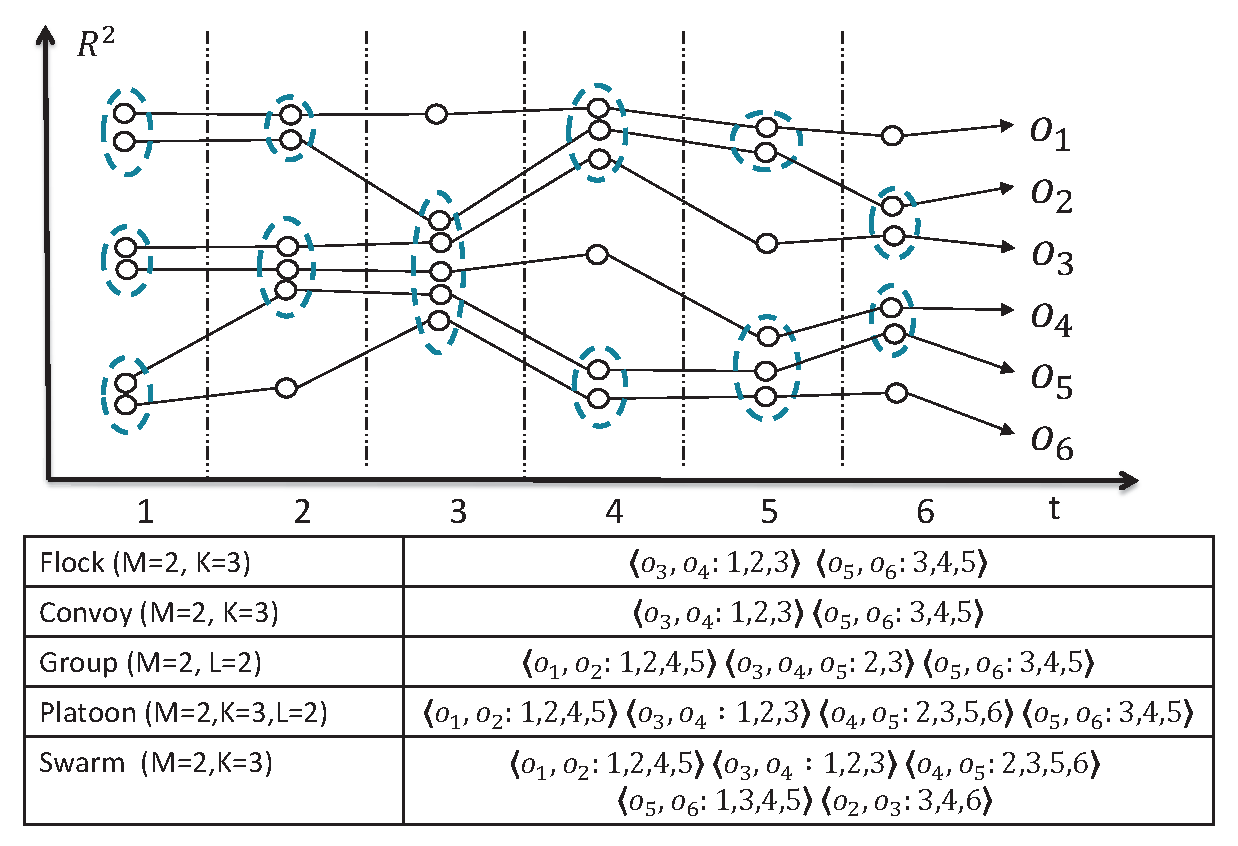
\includegraphics[width=\textwidth]{chapter5/related_work.eps}
\caption{Trajectories and co-movement patterns. The example consists of six trajectories across six snapshots. Objects in spatial clusters are enclosed by dotted circles. $M$ is the minimum cluster cardinality; $K$ denotes the minimum number of snapshots for the occurrence of a spatial cluster; and $L$ denotes the minimum length for local consecutiveness.}
\label{fig:related_work}
\end{figure}

Figure~\ref{fig:related_work} is an example to demonstrate the concepts of the various co-movement patterns. The trajectory database consists of six moving objects and the temporal dimension is discretized into six snapshots. In each snapshot, we treat the clustering method as a blackbox and assume that they generate the same clusters. Objects in proximity are grouped in the dotted circles. As aforementioned, there are three parameters to determine the co-movement patterns and the default settings in this example are $M=2$, $K=3$ and $L=2$. Both the \emph{flock} and the \emph{convoy} require the spatial clusters to last for at least $K$ consecutive  timestamps. Hence, $\langle o_3,o_4:1,2,3 \rangle$ and $\langle o_5,o_6:3,4,5 \rangle$  are the only two candidates matching the patterns. The \textit{swarm} relaxes the pattern matching by discarding the temporal consecutiveness constraint. Thus, it generates many more candidates than the \textit{flock} and the \textit{convoy}. The \textit{group} and the \textit{platoon} add another constraint on local consecutiveness to retain meaningful patterns. For instance, $\langle o_1,o_2:1,2,4,5 \rangle$ is a pattern matching local consecutiveness because timestamps $(1,2)$ and $(4,5)$ are two segments with length no smaller than $L=2$. The difference between the \textit{group} and the \textit{platoon} is that the \textit{platoon} has an additional parameter $K$ to specify the minimum number of snapshots for the spatial clusters. This explains why $\langle o_3,o_4,o_5:2,3 \rangle$ is a  \textit{group} pattern but not a \textit{platoon} pattern.

As can be seen, there are various co-movement patterns requested by different applications and it is cumbersome to design a tailored solution for each type. In addition, despite the generality of the \emph{platoon} (i.e., it can be reduced to other types of patterns via proper parameter settings), it suffers from the so-called \emph{loose-connection} anomaly. We use two objects $o_1$ and $o_2$ in Figure~\ref{fig:platoon_weakpoint} to illustrate the scenario. These two objects form a \emph{platoon} pattern in timestamps $(1,2,3,102,103,104)$. However, the two consecutive segments are $98$ timestamps apart, resulting in a false positive co-movement pattern. In reality, such an anomaly may be caused  by the periodic movements of unrelated objects, such as vehicles stopping at the same petrol station or animals pausing at the same water source. 
Unfortunately, none of the existing patterns have directly addressed this anomaly.

\begin{figure}[h]
\center
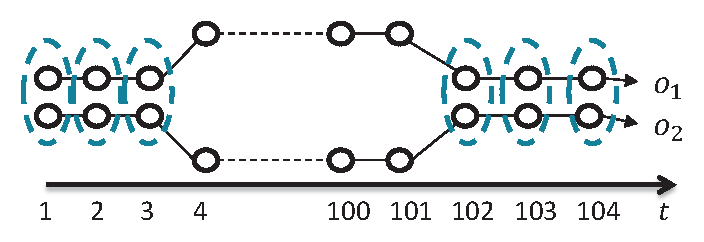
\includegraphics[width=0.8\textwidth]{chapter5/platoon_weakpoint.eps}
%\vspace{-0.5em}
\caption{\emph{Loose-connection} anomaly. Even though $\langle o_1, o_2\rangle$ is considered as a valid \emph{platoon} pattern, it is highly probable that these two objects are not related as the two consecutive segments  are 98 timestamps apart. 
}
%%\vspace{-0.5em}
\label{fig:platoon_weakpoint}
\end{figure}



The other issue with existing methods is that they are built on top of centralized indexes. Thus, they may not be scalable to handle real large-scale trajectories collected by today's
positioning technologies.
%As the collection of trajectories has been drastically boosted by advanced positioning technologies, centralized solutions are becoming limited for large-scale trajectories.
%
% With tremendous  With the prevalence of positioning devices, the scale and spectrum 
%of the trajectory collection has been drastically boosted to
%an unprecedented level. Tremendous amounts of trajectories are continually being generated from animal telemetry chips, 
%vehicle GPSs and wearable devices.
%
% which may not be scalable. 
Table~\ref{tbl:existing_co_patterns} shows their theoretical complexities in the worst cases and the largest real dataset ever evaluated in previous studies is up to million-scale points collected from hundreds of moving objects. In practice, the dataset is of much higher scale and the scalability of existing methods is left unknown. Thus, we conduct an experimental evaluation with $4000$ objects moving for $2500$ timestamps to examine the scalability. Results in Figure~\ref{fig:related_work_scalability} show that their performances degrade dramatically as the dataset scales up. For instance, the detection time of \emph{group} drops twenty times as the number of objects grows from \emph{1k} to \emph{4k}. Similarly,
the performance of \emph{swarm} drops over fifteen times as the number of snapshots grows from \emph{1k} to \emph{2.5k}.
These observations imply that existing methods are not scalable to support large-scale trajectory databases. 

\begin{figure}[h]
    \centering
    \begin{subfigure}[b]{0.45\textwidth}
            \centering
            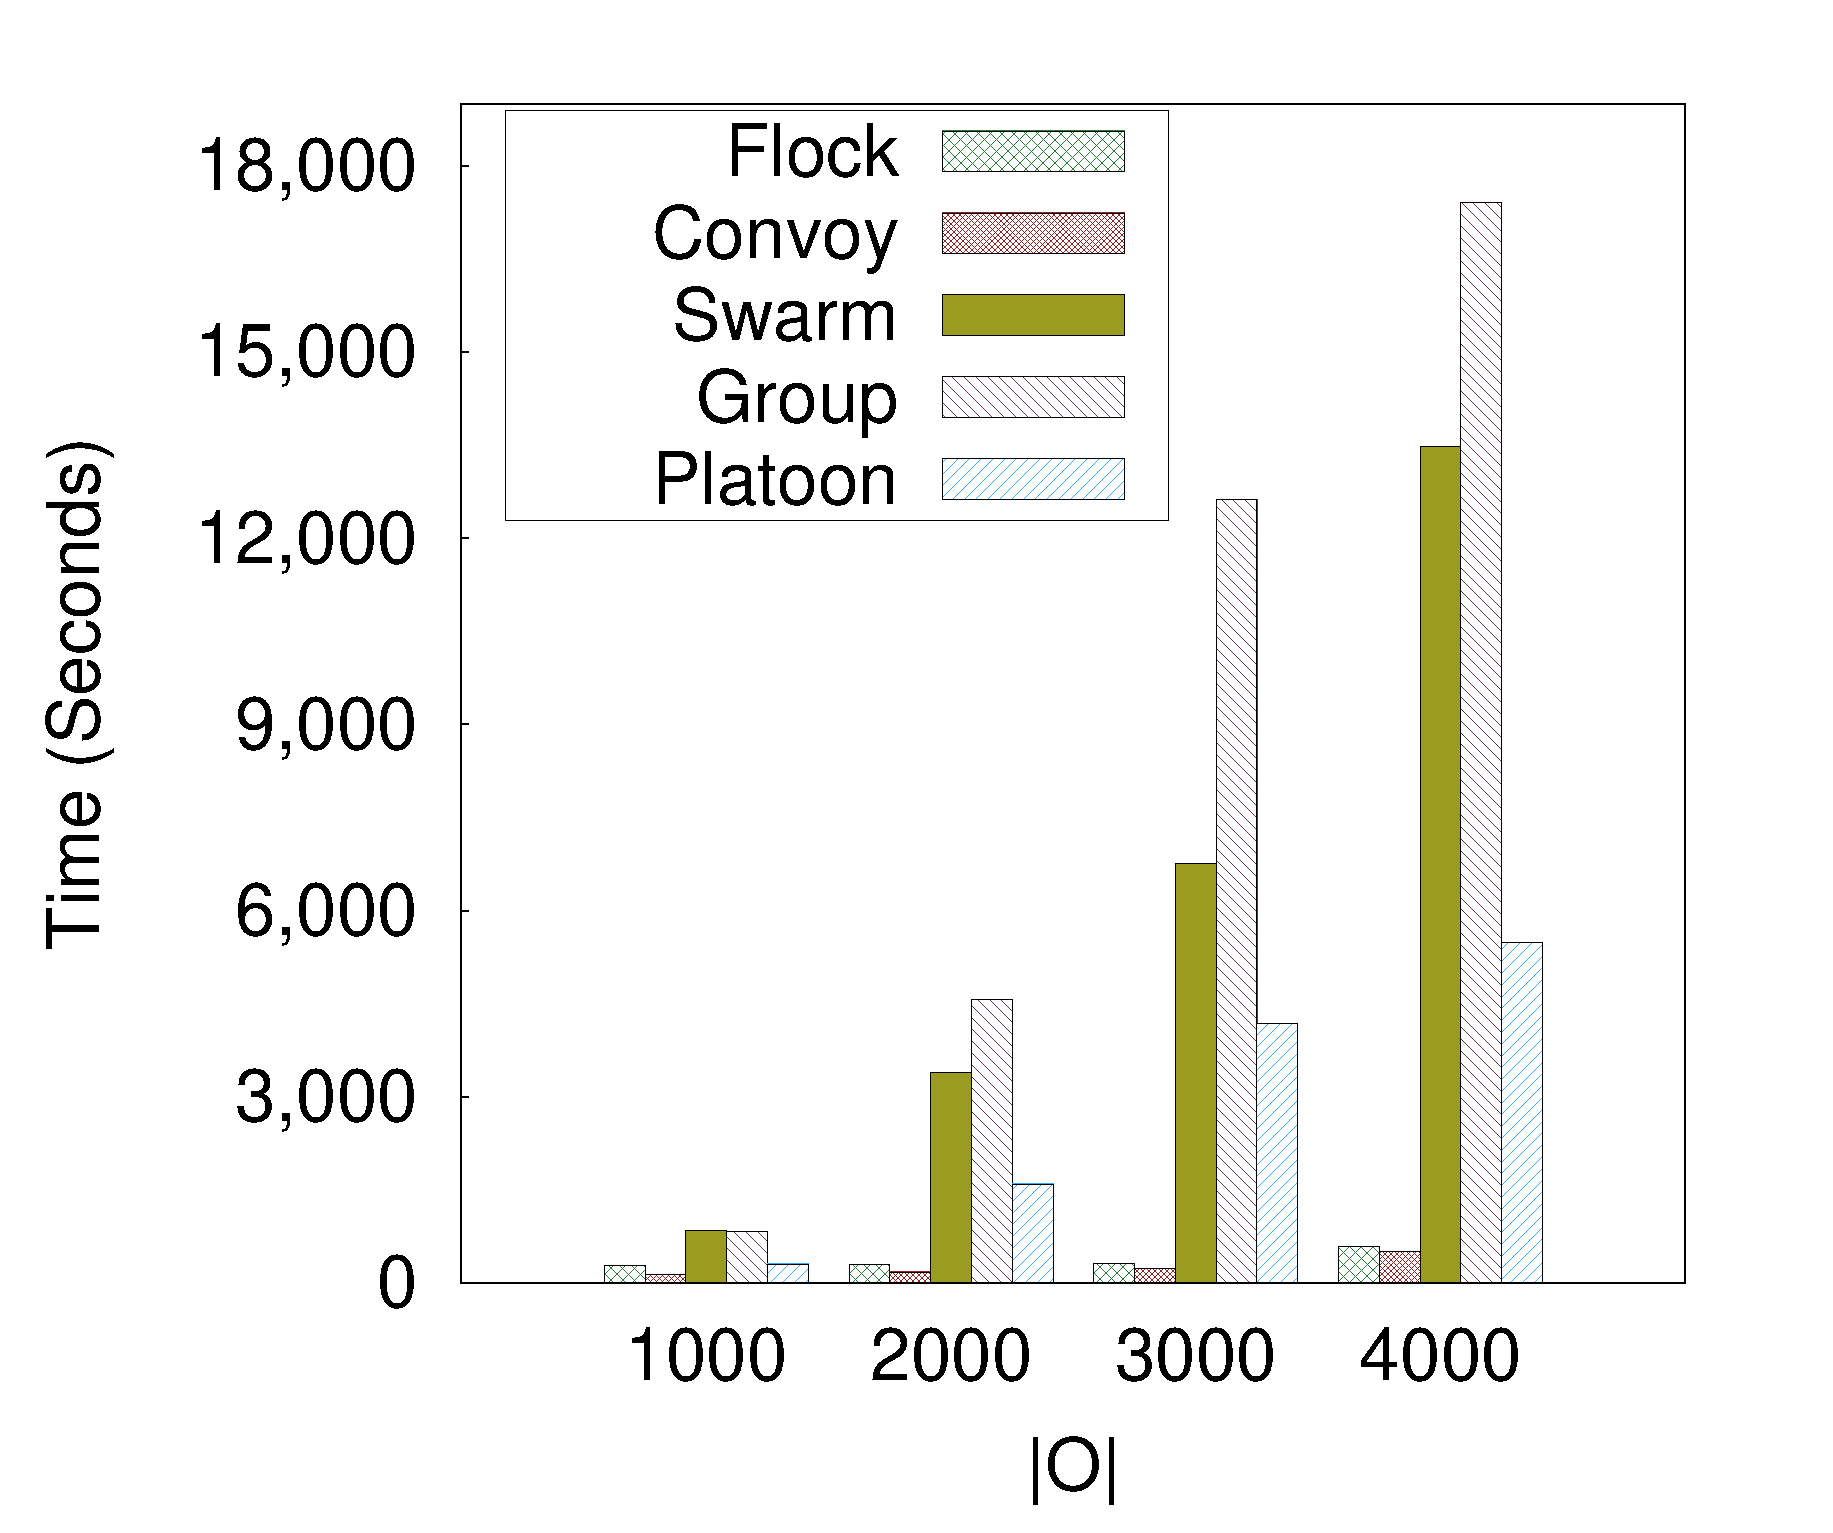
\includegraphics[width=\textwidth]{chapter5/rw_perf_O.eps}
		\subcaption{Varying No.~of objects} 
    \label{fig:fig1}
    \end{subfigure}
    \begin{subfigure}[b]{0.45\textwidth}
            \centering
            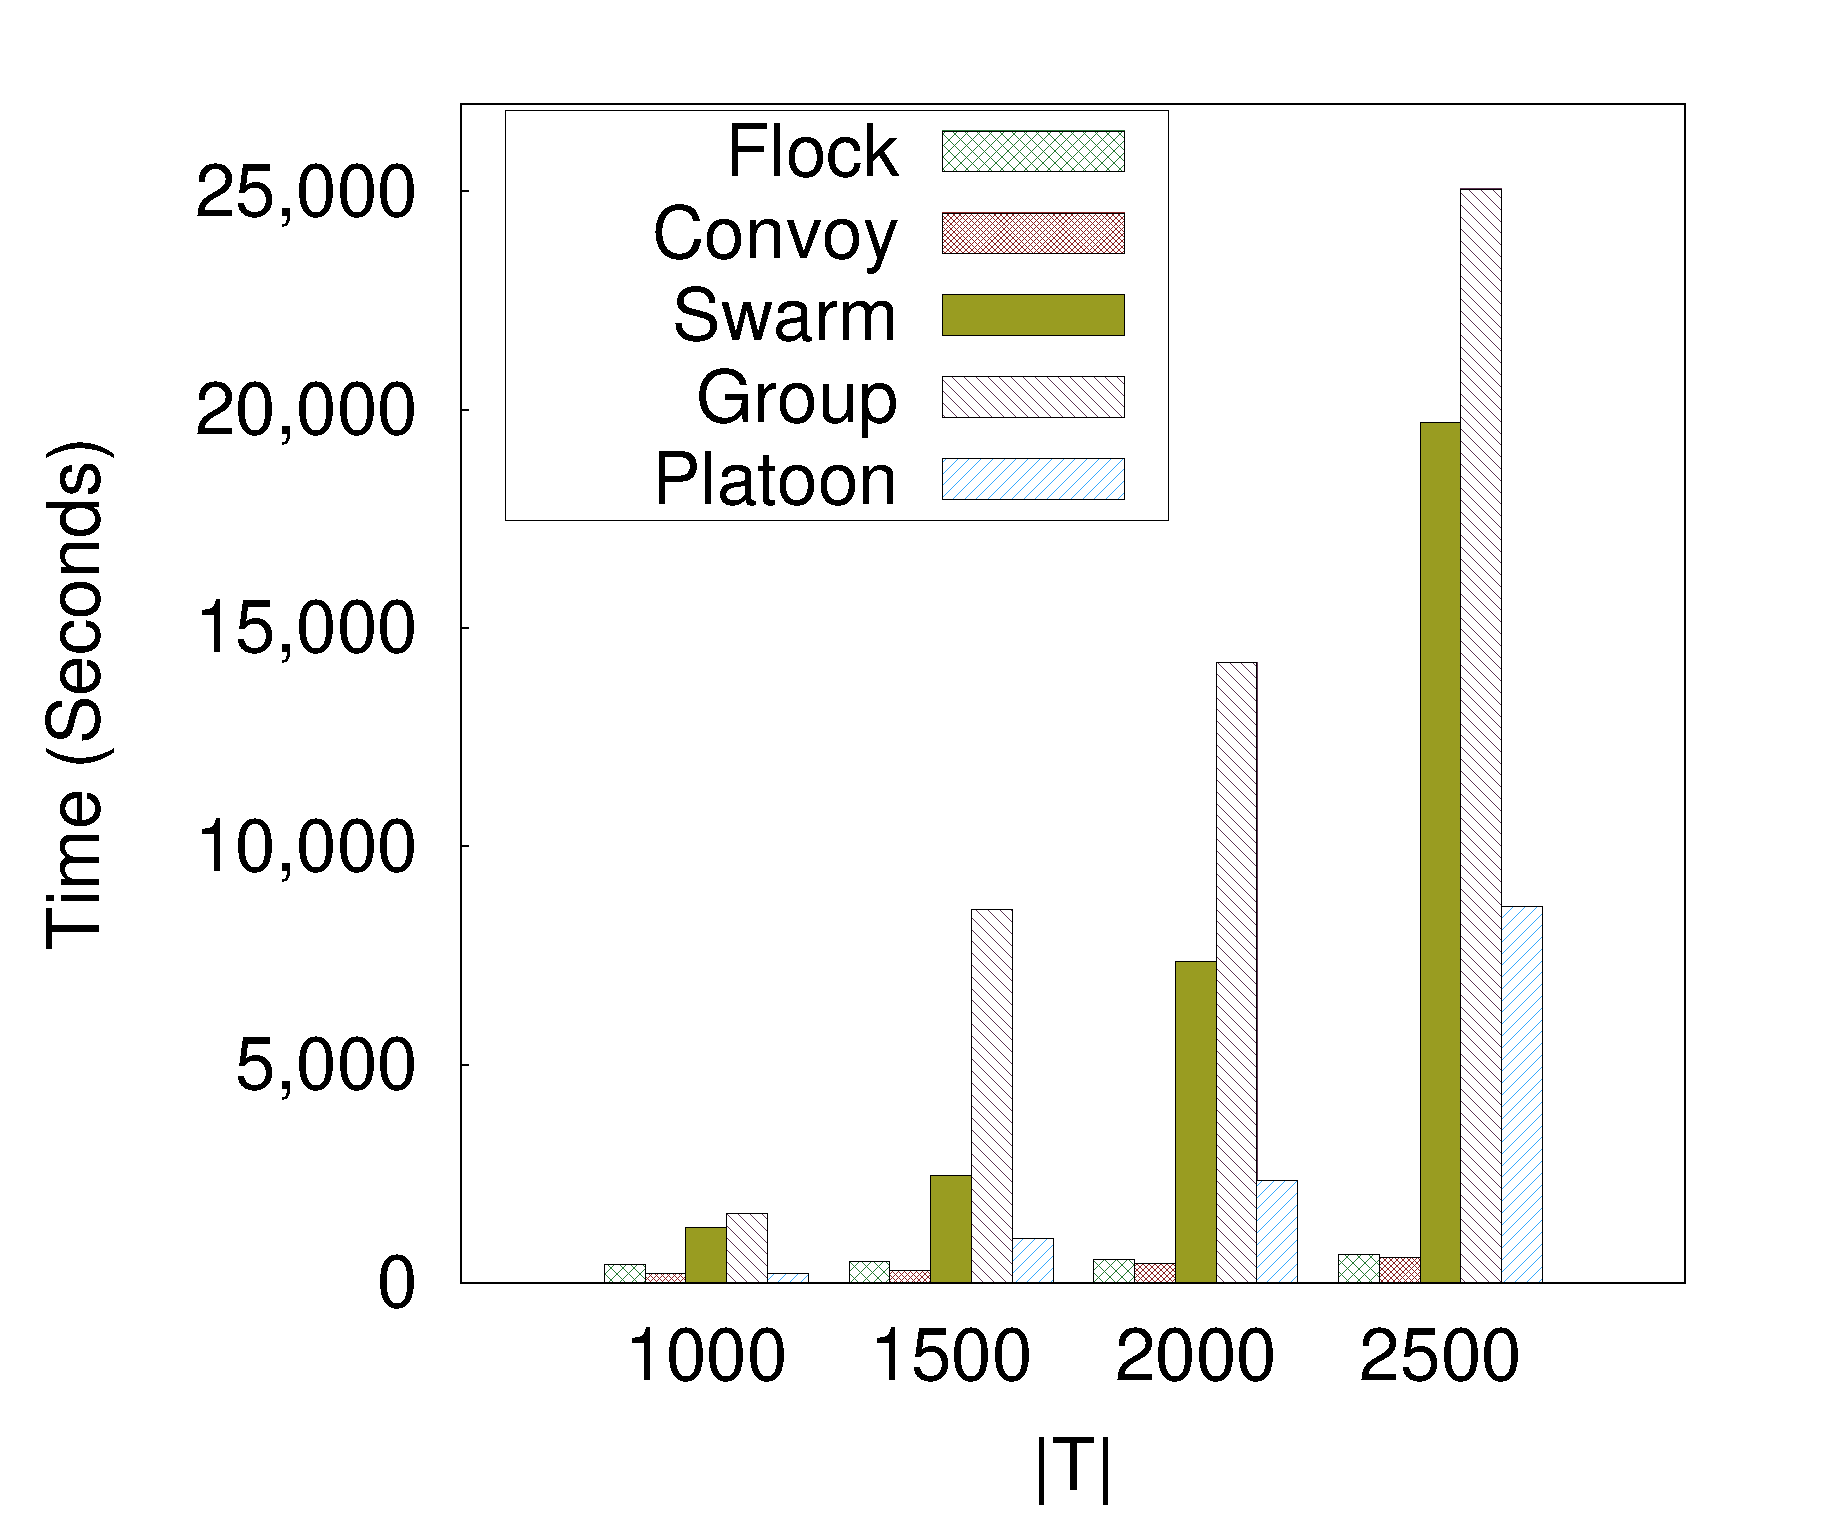
\includegraphics[width=\textwidth]{chapter5/rw_perf_T.eps}
         \subcaption{Varying No.~of timestamps}
    \label{fig:fig2}
    \end{subfigure}
    %\vspace{-0.5em}
    \caption{Performance measures on existing co-movement patterns. A sampled GeoLife dataset
    is used with up to 2.4 million data points. Default parameters are $M=15$, $K=180$, $L=30$.}
    %\vspace{-0.5em}
    \label{fig:related_work_scalability}
\end{figure}
%
%Therefore, in this paper, our contributions are closing
%these two gaps.
%
%to close these two gaps.
%
%Therefore, in this paper, our aim is to close these two gaps 
%via the following contributions.
%we aim to close these two gaps by making two contributions. 
In this chapter, we close these two gaps by making the following contributions.
First, we propose the \emph{general co-movement pattern} (GCMP) which models
various co-moment patterns in a unified way and can avoid 
the \emph{loose-connection} anomaly. In GCMP,
we introduce a new gap parameter $G$ to pose a constraint on the temporal gap between two consecutive segments. 
By setting a feasible $G$, the loose-connection anomaly can be effectively controlled. In addition, our GCMP is also general. It can be reduced to any of the previous pattern by customizing its parameters.

Second, we investigate deploying our GCMP detector on the modern MapReduce platform (i.e., Apache Spark) to tackle the scalability issue. Our technical contributions are threefold. First, we design a baseline solution by replicating the snapshots 
%in multiple data chunks 
to support effective parallel mining. 
Second, we devise a novel \emph{Star Partitioning and ApRiori Enumerator} (SPARE) framework to resolve limitations of the baseline. 
SPARE achieves workload balance by partitioning objects into fine granular stars. 
For each partition, an Apriori Enumerator is adopted to mine the co-movement patterns. 
Third, we leverage the \emph{temporal monotonicity} property of GCMP 
to design several optimization techniques including \emph{sequence simplification}, \emph{monotonicity pruning} and \emph{forward closure check} to further reduce the number of candidates enumerated in SPARE.

We conduct a set of extensive experiments on three large-scale real datasets with hundreds of millions of
temporal points. 
The results show that both our parallel schemes efficiently support GCMP mining in large datasets.
In particular, with over 170 million trajectory points,
SPARE achieves up to 112 times speedup using 162 cores as compared to the state-of-the-art centralized schemes.
Moreover, SPARE further achieves almost linear scalability with upto 14 times efficiency
as compared to the baseline algorithm.

%The rest of our paper is organized as follows: Section~\ref{sec:related_works} summarizes the relevant literature on 
%trajectory pattern mining. Section~\ref{sec:definition} states the problem of general co-movement pattern mining. Section~\ref{sec:trm} provides a baseline %solution named \emph{Temporal Replication and Parallel %Mining} (TRPM). An advanced solution named
%\emph{Star Partitioning and ApRiori Enumerator} (SPARE) is presented in Section~\ref{sec:spm}. Section~\ref{sec:exp} conducts extensive experiments to verify the efficiency of our solutions. Finally, Section~\ref{sec:concl} concludes the paper.

The rest of this chapter is organized as follows: %Section~\ref{sec:related_works} summarizes related work. 
Section~\ref{sec:definition} states the problem of general co-movement pattern mining. Section~\ref{sec:trm} provides a baseline 
solution. % named \emph{Temporal Replication and Parallel Mining} (TRPM).
An advanced solution named
\emph{Star Partitioning and ApRiori Enumerator} (SPARE) is presented in Section~\ref{sec:spm}. Section~\ref{sec:exp} reports our experimental evaluation.
Finally, Section~\ref{sec:concl} summarizes this chapter.